\chapter{Verkon läpikäynti}

Syvyyshaku ja leveyshaku ovat keskeisiä
menetelmiä verkon läpikäyntiin.
Molemmat algoritmit lähtevät liikkeelle
tietystä verkon solmusta ja 
käyvät läpi kaikki solmut,
joihin aloitussolmusta pääsee.
Algoritmien erona on,
missä järjestyksessä ne etenevät verkon solmuja.

\section{Syvyyshaku}

Syvyyshaku (\textit{depth-first search})
on suoraviivainen menetelmä verkon läpikäyntiin.
Syvyyshaku lähtee liikkeelle tietystä
verkon solmusta ja etenee siitä
kaikkiin solmuihin, jotka ovat
saavutettavissa kaaria kulkemalla.

Syvyyshaku etenee verkossa syvyyssuuntaisesti
eli valitsee aina yhden suunnan
ja kulkee eteenpäin niin kauan
kuin vastaan tulee uusia solmuja.
Tämän jälkeen haku perääntyy kokeilemaan
muita suuntia.
Haku pitää kirjaa vierailemistaan solmuista,
jotta se käsittelee kunkin solmun vain kerran.

\subsubsection*{Toiminta}

Tarkastellaan syvyyshaun toimintaa
seuraavassa verkossa:
\begin{center}
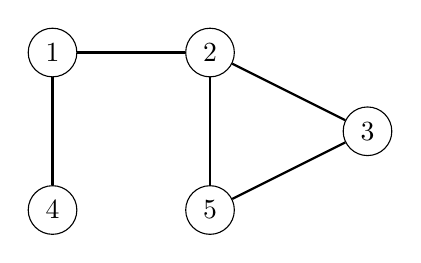
\begin{tikzpicture}
\node[draw, circle] (1) at (1,5) {$1$};
\node[draw, circle] (2) at (3,5) {$2$};
\node[draw, circle] (3) at (5,4) {$3$};
\node[draw, circle] (4) at (1,3) {$4$};
\node[draw, circle] (5) at (3,3) {$5$};

\path[draw,thick,-] (1) -- (2);
\path[draw,thick,-] (2) -- (3);
\path[draw,thick,-] (1) -- (4);
\path[draw,thick,-] (3) -- (5);
\path[draw,thick,-] (2) -- (5);
\end{tikzpicture}
\end{center}
Syvyyshaku voi lähteä liikkeelle
mistä tahansa solmusta,
mutta oletetaan nyt,
että haku lähtee liikkeelle solmusta 1.

Solmun 1 naapurit ovat solmut 2 ja 4,
joista haku etenee ensin solmuun 2:
\begin{center}
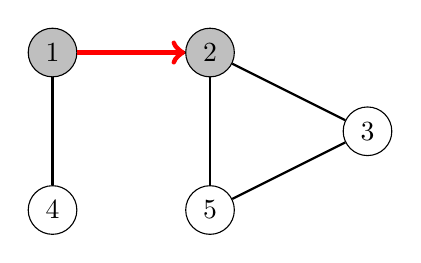
\begin{tikzpicture}
\node[draw, circle,fill=lightgray] (1) at (1,5) {$1$};
\node[draw, circle,fill=lightgray] (2) at (3,5) {$2$};
\node[draw, circle] (3) at (5,4) {$3$};
\node[draw, circle] (4) at (1,3) {$4$};
\node[draw, circle] (5) at (3,3) {$5$};

\path[draw,thick,-] (1) -- (2);
\path[draw,thick,-] (2) -- (3);
\path[draw,thick,-] (1) -- (4);
\path[draw,thick,-] (3) -- (5);
\path[draw,thick,-] (2) -- (5);

\path[draw=red,thick,->,line width=2pt] (1) -- (2);
\end{tikzpicture}
\end{center}
Tämän jälkeen haku etenee vastaavasti
solmuihin 3 ja 5:
\begin{center}
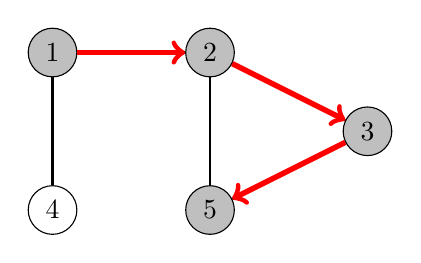
\begin{tikzpicture}
\node[draw, circle,fill=lightgray] (1) at (1,5) {$1$};
\node[draw, circle,fill=lightgray] (2) at (3,5) {$2$};
\node[draw, circle,fill=lightgray] (3) at (5,4) {$3$};
\node[draw, circle] (4) at (1,3) {$4$};
\node[draw, circle,fill=lightgray] (5) at (3,3) {$5$};

\path[draw,thick,-] (1) -- (2);
\path[draw,thick,-] (2) -- (3);
\path[draw,thick,-] (1) -- (4);
\path[draw,thick,-] (3) -- (5);
\path[draw,thick,-] (2) -- (5);

\path[draw=red,thick,->,line width=2pt] (1) -- (2);
\path[draw=red,thick,->,line width=2pt] (2) -- (3);
\path[draw=red,thick,->,line width=2pt] (3) -- (5);
\end{tikzpicture}
\end{center}
Solmun 5 naapurit ovat 2 ja 3,
mutta haku on käynyt jo molemmissa,
joten on aika peruuttaa taaksepäin.
Myös solmujen 3 ja 2 naapurit on käyty,
joten haku peruuttaa solmuun 1 asti.
Siitä lähtee kaari, josta pääsee
solmuun 4:
\begin{center}
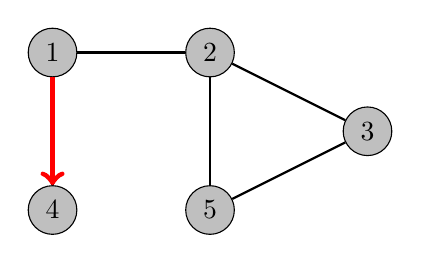
\begin{tikzpicture}
\node[draw, circle,fill=lightgray] (1) at (1,5) {$1$};
\node[draw, circle,fill=lightgray] (2) at (3,5) {$2$};
\node[draw, circle,fill=lightgray] (3) at (5,4) {$3$};
\node[draw, circle,fill=lightgray] (4) at (1,3) {$4$};
\node[draw, circle,fill=lightgray] (5) at (3,3) {$5$};

\path[draw,thick,-] (1) -- (2);
\path[draw,thick,-] (2) -- (3);
\path[draw,thick,-] (1) -- (4);
\path[draw,thick,-] (3) -- (5);
\path[draw,thick,-] (2) -- (5);

\path[draw=red,thick,->,line width=2pt] (1) -- (4);
\end{tikzpicture}
\end{center}
Tämän jälkeen haku päättyy,
koska se on käynyt kaikissa solmuissa.

Syvyyshaun aikavaativuus on $O(n+m)$,
missä $n$ on solmujen määrä ja $m$ on kaarten määrä,
koska haku käsittelee kerran jokaisen solmun ja kaaren.

\subsubsection*{Toteutus}

Syvyyshaku on yleensä mukavinta toteuttaa
rekursiolla.
Seuraava funktio \texttt{dfs}
suorittaa syvyyshaun sille parametrina
annetusta solmusta lähtien.
Funktio olettaa, että
verkko on tallennettu vieruslistoina
taulukkoon
\begin{lstlisting}
vector<int> v[N];
\end{lstlisting}
ja pitää lisäksi yllä taulukkoa
\begin{lstlisting}
int z[N];
\end{lstlisting}
joka kertoo, missä solmuissa haku on käynyt.
Alussa taulukon jokainen arvo on 0,
ja kun haku saapuu solmuun $s$,
sen kohdalle merkitään luku 1.
Funktion toteutus on seuraavanlainen:
\begin{lstlisting}
void dfs(int s) {
    if (z[s]) return;
    z[s] = 1;
    // solmun s käsittely tähän
    for (int i = 0; i < v[s].size(); i++) {
        dfs(v[s][i]);
    }
}
\end{lstlisting}

\section{Leveyshaku}

Leveyshaku (\textit{breadth-first search})
käy solmut läpi järjestyksessä sen mukaan,
kuinka kaukana ne ovat aloitussolmusta.
Niinpä leveyshaun avulla pystyy laskemaan
etäisyyden aloitussolmusta kaikkiin
muihin solmuihin.
Leveyshaku on kuitenkin vaikeampi
toteuttaa kuin syvyyshaku.

Leveyshakua voi ajatella niin,
että se käy solmuja läpi kerros kerrallaan.
Ensin haku käy läpi solmut,
joihin pääsee yhdellä kaarella
alkusolmusta.
Tämän jälkeen vuorossa ovat
solmut, joihin pääsee kahdella
kaarella alkusolmusta jne.
Sama jatkuu, kunnes uusia käsiteltäviä
solmuja ei enää ole.

\subsubsection*{Toiminta}

Tarkastellaan leveyshaun toimintaa
seuraavassa verkossa:

\begin{center}
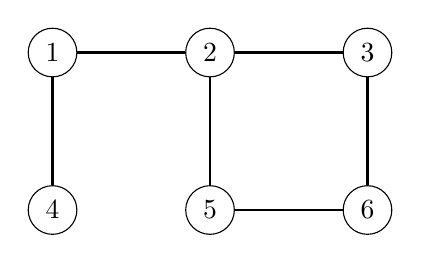
\begin{tikzpicture}
\node[draw, circle] (1) at (1,5) {$1$};
\node[draw, circle] (2) at (3,5) {$2$};
\node[draw, circle] (3) at (5,5) {$3$};
\node[draw, circle] (4) at (1,3) {$4$};
\node[draw, circle] (5) at (3,3) {$5$};
\node[draw, circle] (6) at (5,3) {$6$};


\path[draw,thick,-] (1) -- (2);
\path[draw,thick,-] (2) -- (3);
\path[draw,thick,-] (1) -- (4);
\path[draw,thick,-] (3) -- (6);
\path[draw,thick,-] (2) -- (5);
\path[draw,thick,-] (5) -- (6);
\end{tikzpicture}
\end{center}
Oletetaan jälleen,
että haku alkaa solmusta 1.
Haku etenee ensin kaikkiin solmuihin,
joihin pääsee alkusolmusta:
\\
\begin{center}
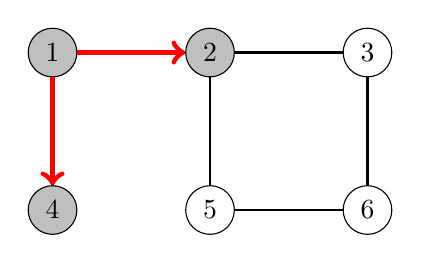
\begin{tikzpicture}
\node[draw, circle,fill=lightgray] (1) at (1,5) {$1$};
\node[draw, circle,fill=lightgray] (2) at (3,5) {$2$};
\node[draw, circle] (3) at (5,5) {$3$};
\node[draw, circle,fill=lightgray] (4) at (1,3) {$4$};
\node[draw, circle] (5) at (3,3) {$5$};
\node[draw, circle] (6) at (5,3) {$6$};

\path[draw,thick,-] (1) -- (2);
\path[draw,thick,-] (2) -- (3);
\path[draw,thick,-] (1) -- (4);
\path[draw,thick,-] (3) -- (6);
\path[draw,thick,-] (2) -- (5);
\path[draw,thick,-] (5) -- (6);

\path[draw,thick,-] (1) -- (2);
\path[draw,thick,-] (2) -- (3);
\path[draw,thick,-] (1) -- (4);
\path[draw,thick,-] (2) -- (5);

\path[draw=red,thick,->,line width=2pt] (1) -- (2);
\path[draw=red,thick,->,line width=2pt] (1) -- (4);
\end{tikzpicture}
\end{center}
Seuraavaksi haku etenee solmuihin 3 ja 5:
\\
\begin{center}
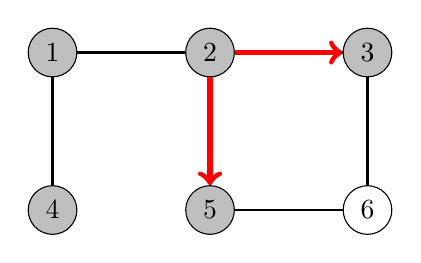
\begin{tikzpicture}
\node[draw, circle,fill=lightgray] (1) at (1,5) {$1$};
\node[draw, circle,fill=lightgray] (2) at (3,5) {$2$};
\node[draw, circle,fill=lightgray] (3) at (5,5) {$3$};
\node[draw, circle,fill=lightgray] (4) at (1,3) {$4$};
\node[draw, circle,fill=lightgray] (5) at (3,3) {$5$};
\node[draw, circle] (6) at (5,3) {$6$};

\path[draw,thick,-] (1) -- (2);
\path[draw,thick,-] (2) -- (3);
\path[draw,thick,-] (1) -- (4);
\path[draw,thick,-] (3) -- (6);
\path[draw,thick,-] (2) -- (5);
\path[draw,thick,-] (5) -- (6);

\path[draw,thick,-] (1) -- (2);
\path[draw,thick,-] (2) -- (3);
\path[draw,thick,-] (1) -- (4);
\path[draw,thick,-] (2) -- (5);

\path[draw=red,thick,->,line width=2pt] (2) -- (3);
\path[draw=red,thick,->,line width=2pt] (2) -- (5);
\end{tikzpicture}
\end{center}
Viimeisenä haku etenee solmuun 6:
\\
\begin{center}
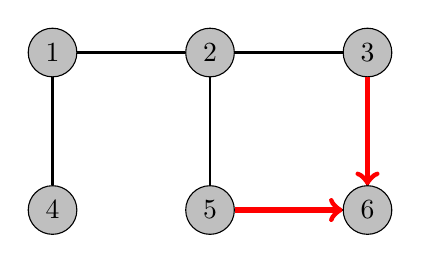
\begin{tikzpicture}
\node[draw, circle,fill=lightgray] (1) at (1,5) {$1$};
\node[draw, circle,fill=lightgray] (2) at (3,5) {$2$};
\node[draw, circle,fill=lightgray] (3) at (5,5) {$3$};
\node[draw, circle,fill=lightgray] (4) at (1,3) {$4$};
\node[draw, circle,fill=lightgray] (5) at (3,3) {$5$};
\node[draw, circle,fill=lightgray] (6) at (5,3) {$6$};

\path[draw,thick,-] (1) -- (2);
\path[draw,thick,-] (2) -- (3);
\path[draw,thick,-] (1) -- (4);
\path[draw,thick,-] (3) -- (6);
\path[draw,thick,-] (2) -- (5);
\path[draw,thick,-] (5) -- (6);

\path[draw,thick,-] (1) -- (2);
\path[draw,thick,-] (2) -- (3);
\path[draw,thick,-] (1) -- (4);
\path[draw,thick,-] (2) -- (5);

\path[draw=red,thick,->,line width=2pt] (3) -- (6);
\path[draw=red,thick,->,line width=2pt] (5) -- (6);
\end{tikzpicture}
\end{center}
Leveyshaun tuloksena selviää etäisyys
kuhunkin verkon solmuun alkusolmusta.
Etäisyys on sama kuin kerros,
jossa solmu käsiteltiin haun aikana:

\begin{tabular}{ll}
\\
solmu & etäisyys \\
\hline
1 & 0 \\
2 & 1 \\
3 & 2 \\
4 & 1 \\
5 & 2 \\
6 & 3 \\
\\
\end{tabular}

Leveyshaun aikavaativuus on syvyyshaun tavoin $O(n+m)$,
missä $n$ on solmujen määrä ja $m$ on kaarten määrä.

\subsubsection*{Toteutus}

Leveyshaun toteutus on syvyyshakua monimutkaisempi,
koska haku käy läpi solmuja verkon eri
puolilta niiden etäisyyden mukaan.
Tyypillinen toteutus on pitää yllä jonoa
käsiteltävistä solmuista.
Joka askeleella otetaan käsittelyyn seuraava
solmu jonosta ja uudet solmut lisätään
jonon perälle.

Seuraava koodi toteuttaa leveyshaun
solmusta $s$ lähtien.
Koodi olettaa, että verkko on tallennettu
vieruslistoina, ja pitää yllä jonoa
\begin{lstlisting}
queue<int> q;
\end{lstlisting}
joka sisältää solmut käsittelyjärjestyksessä.
Koodi lisää aina uudet vastaan tulevat solmut
jonon perään ja ottaa seuraavaksi käsiteltävän
solmun jonon alusta,
minkä ansiosta solmut käsitellään tasoittain
alkusolmusta lähtien.

Lisäksi koodi käyttää taulukoita
\begin{lstlisting}
int z[N], e[N];
\end{lstlisting}
niin, että taulukko \texttt{z} sisältää tiedon,
missä solmuissa haku on käynyt,
ja taulukkoon \texttt{e} lasketaan lyhin
etäisyys alkusolmusta kaikkiin verkon solmuihin.
Toteutuksesta tulee seuraavanlainen:
\begin{lstlisting}
q.push(s);
z[s] = 1; e[s] = 0;
while (!q.empty()) {
    int s = q.front(); q.pop();
    // solmun s käsittely tähän     
    for (int i = 0; i < v[s].size(); i++) {
        int u = v[s][i];
        if (z[u]) continue;
        z[u] = 1; e[u] = e[s]+1;
        q.push(u);
    }
}
\end{lstlisting}

\section{Sovelluksia}

Verkon läpikäyntien avulla
saa selville monia asioita
verkon rakenteesta.
Seuraavissa sovelluksissa
voi käyttää joko
syvyyshakua tai leveyshakua,
mutta syvyyshaku
on käytännössä parempi valinta,
koska sen toteutus on helpompi.

\subsubsection{Yhtenäisyys}

Verkko on yhtenäinen,
jos mistä tahansa solmuista
pääsee kaikkiin muihin solmuihin.
Niinpä verkon yhtenäisyys selviää
aloittamalla läpikäynti
jostakin verkon solmusta ja
tarkastamalla, pääseekö siitä kaikkiin solmuihin.
Jos kaikki solmut
tulevat vastaan läpikäynnin aikana,
niin verkko on yhtenäinen.

\subsubsection{Komponentit}

Jos verkko ei ole yhtenäinen,
se muodostuu useammasta komponentista.
Kaikki tiettyyn komponenttiin kuuluvat
solmut löytyvät aloittamalla
läpikäynti jostakin komponentin solmusta.

Verkon komponentit saa selville
käymällä läpi verkon solmut ja
pitämällä kirjaa komponenteista.
Jos solmu ei kuulu vielä
komponenttiin, se aloittaa uuden
komponentin, johon kuuluvat kaikki
solmut, joihin solmusta pääsee.

\subsubsection{Syklin etsiminen}

Suuntaamaton verkko sisältää syklin,
jos verkon läpikäynnin aikana tulee vastaan
solmu, jossa on käyty jo aiemmin,
ja tämä solmu on jokin muu kuin se solmu,
jonka kautta nykyiseen solmuun tultiin.

Syklin olemassaolon voi myös päätellä
komponentin koosta. Jos komponentin
kaarten määrä on yhtä pienempi kuin
solmujen määrä, komponentissa ei ole sykliä,
ja jos kaarten määrä on tätä suurempi,
komponentissa on sykli.

\subsubsection{Kaksijakoisuus}

Verkko on kaksijakoinen,
jos sen solmut voi värittää
kahdella värillä
niin, että kahta samanväristä
solmua ei ole vierekkäin.
Kaksijakoisuus on yllättävän
helppoa selvittää
verkon läpikäynnin avulla.

Ideana on värittää alkusolmu
siniseksi, sen kaikki naapurit
punaiseksi, niiden kaikki naapurit
siniseksi, jne.
Jos jossain vaiheessa
ilmenee ristiriita
(saman solmun tulisi olla sekä
sininen että punainen),
verkko ei ole kaksijakoinen.
Muuten verkko on kaksijakoinen
ja yksi väritys on muodostunut.

Tämä algoritmi toimii,
koska kun värejä on vain kaksi,
ensimmäisen solmun värin valinta
määrittää kaikkien muiden
samassa komponentissa olevien
solmujen värin.
Ei ole merkitystä,
kumman värin ensimmäinen
solmu saa.

Yleensä ottaen on vaikea ongelma
selvittää, voiko verkon solmuja
värittää $k$ värillä niin,
ettei missään kohtaa ole vierekkäin
kahta samanväristä solmua.
Edes tapaukseen $k=3$ ei tunneta
mitään tehokasta algoritmia.

\section{Labyrintin käsittely}

Labyrintti on ruudukko, joka muodostuu lattia- ja seinäruuduista,
ja labyrintissa on sallittua kulkea lattiaruutuja pitkin.
Labyrinttia
\begin{center}
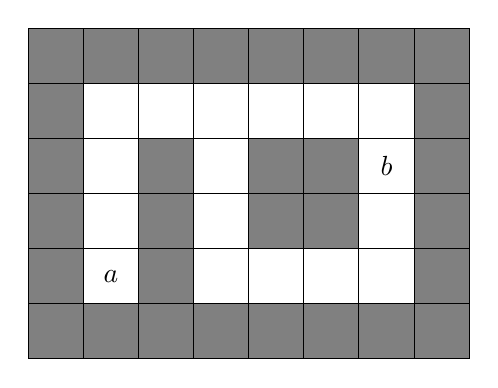
\begin{tikzpicture}[scale=0.7]
\fill[color=gray] (0,0) rectangle (8,1);
\fill[color=gray] (0,5) rectangle (8,6);
\fill[color=gray] (0,0) rectangle (1,6);
\fill[color=gray] (7,0) rectangle (8,6);

\fill[color=gray] (2,0) rectangle (3,4);
\fill[color=gray] (4,2) rectangle (6,4);

\draw (0,0) grid (8,6);

\node at (1.5,1.5) {$a$};
\node at (6.5,3.5) {$b$};
\end{tikzpicture}
\end{center}
vastaa luontevasti verkko
\begin{center}
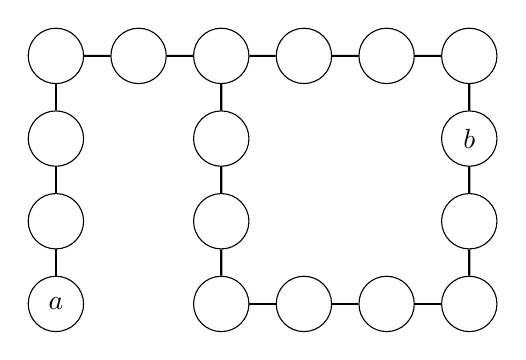
\begin{tikzpicture}[scale=0.7]
\node[draw,circle,minimum size=20pt] (a) at (1,1) {$a$};
\node[draw,circle,minimum size=20pt] (b) at (1,2.5) {};
\node[draw,circle,minimum size=20pt] (c) at (1,4) {};
\node[draw,circle,minimum size=20pt] (d) at (1,5.5) {};
\node[draw,circle,minimum size=20pt] (e) at (2.5,5.5) {};
\node[draw,circle,minimum size=20pt] (f) at (4,5.5) {};
\node[draw,circle,minimum size=20pt] (g) at (5.5,5.5) {};
\node[draw,circle,minimum size=20pt] (h) at (7,5.5) {};
\node[draw,circle,minimum size=20pt] (i) at (8.5,5.5) {};
\node[draw,circle,minimum size=20pt] (j) at (8.5,4) {$b$};
\node[draw,circle,minimum size=20pt] (k) at (8.5,2.5) {};
\node[draw,circle,minimum size=20pt] (l) at (8.5,1) {};
\node[draw,circle,minimum size=20pt] (m) at (7,1) {};
\node[draw,circle,minimum size=20pt] (n) at (5.5,1) {};
\node[draw,circle,minimum size=20pt] (o) at (4,1) {};
\node[draw,circle,minimum size=20pt] (p) at (4,2.5) {};
\node[draw,circle,minimum size=20pt] (q) at (4,4) {};

\path[draw,thick,-] (a) -- (b);
\path[draw,thick,-] (b) -- (c);
\path[draw,thick,-] (c) -- (d);
\path[draw,thick,-] (d) -- (e);
\path[draw,thick,-] (e) -- (f);
\path[draw,thick,-] (f) -- (g);
\path[draw,thick,-] (g) -- (h);
\path[draw,thick,-] (h) -- (i);
\path[draw,thick,-] (i) -- (j);
\path[draw,thick,-] (j) -- (k);
\path[draw,thick,-] (k) -- (l);
\path[draw,thick,-] (l) -- (m);
\path[draw,thick,-] (m) -- (n);
\path[draw,thick,-] (n) -- (o);
\path[draw,thick,-] (o) -- (p);
\path[draw,thick,-] (p) -- (q);
\path[draw,thick,-] (q) -- (f);
\end{tikzpicture}
\end{center}
jossa verkon solmuja ovat labyrintin lattiaruudut
ja solmujen välillä on kaari, jos lattiaruudusta
toiseen pääsee kulkemaan yhdellä askeleella.
Niinpä erilaiset labyrinttiin liittyvät ongelmat
palautuvat verkko-ongelmiksi.

Esimerkiksi syvyyshaulla pystyy selvittämään,
onko ruudusta $a$ reittiä ruutuun $b$
ja leveyshaku kertoo lisäksi,
mikä on pienin mahdollinen askelten määrä reitillä.
Samoin voi esimerkiksi vaikkapa, kuinka monta
toisistaan erillistä huonetta labyrintissa on
sekä kuinka monta ruutua huoneissa on.

Labyrintin tapauksessa ei kannata muodostaa erikseen
verkkoa, vaan syvyyshaun ja leveyshaun voi toteuttaa
suoraan labyrintin ruudukkoon.